\documentclass[11pt,a4paper,oneside]{report}

\usepackage[utf8]{inputenc}
\usepackage[margin=0.5in]{geometry}
\usepackage{amsmath}
\usepackage{tabularx}
\usepackage{listings}
\usepackage{graphicx}
\usepackage[dvipsnames]{xcolor}
\usepackage{textcomp}
\usepackage{float}
\usepackage{hyperref} 
\graphicspath{{img/}}

\renewcommand*\contentsname{Table des matières}
\begin{document}
\lstset{
	language=C++,
	frame=single,
	keywordstyle=\color{blue},
	stringstyle=\color{red},
	commentstyle=\color{OliveGreen},
	morecomment=[l][\color{magenta}]{\#}
}

% ----------------------------------------------------------------------
% begin titlepage

\thispagestyle{empty}
\vspace*{1cm}
\begin{center}
{ \Huge Image Vision Interaction } \\
\vspace*{5mm}
{ \Huge SCI } \\
\vspace*{5mm}
Multi Agent Systems\\
\vspace*{5mm}
Quentin BRAULT
\end{center}

% end titlepage
% ----------------------------------------------------------------------

\begingroup\let\clearpage\relax
\tableofcontents \endgroup

\newpage

\addcontentsline{toc}{section}{Introduction}
\section*{Introduction}
L'architecture et les implémentations ont été réalisées en \textbf{JavaScript}.\\
J'ai choisi Javascript car je voulais pouvoir facilement partager le code et le résultat et je voulais des primitives d'affichage facile d'utilisation. Comme \textbf{JS} s'exécute dans un naviguateur sur n'importe quelle machine et ne demande aucune installation, cela semblait parfait.\\
Et au final, malgrès le fait que le language ne soit pas très orienté objet, j'ai réussis à obtenir des dépendances raisonables et un code propre.

\addcontentsline{toc}{section}{Architecture}
\section*{Architecture}

\begin{center}
Architecture avec attributs et méthodes principales
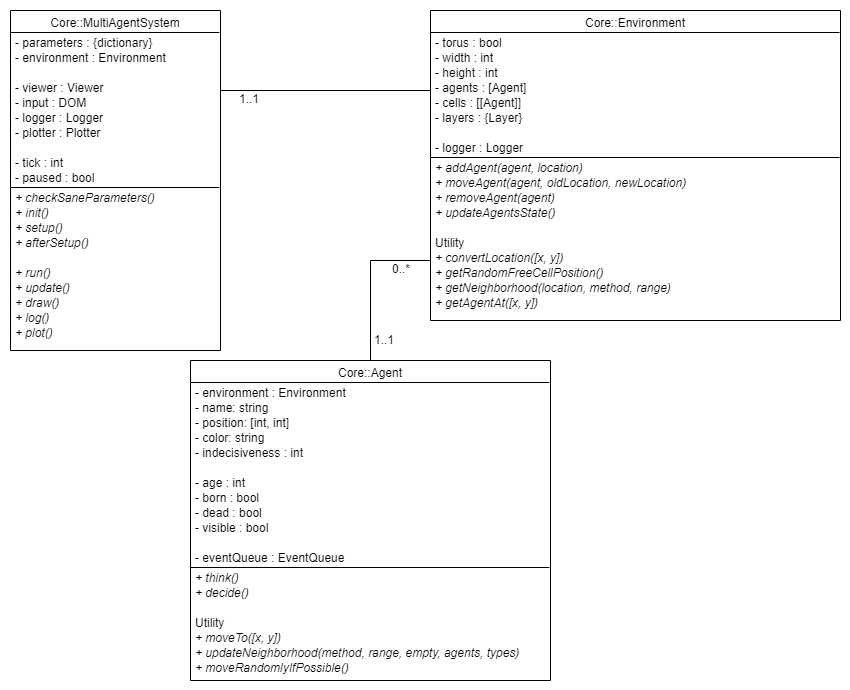
\includegraphics[width=500px]{core}\\
\end{center}

\newpage

\addcontentsline{toc}{subsection}{MultiAgentSystem}
\subsection*{MultiAgentSystem}
La classe \textbf{MultiAgentSystem} va créer l'environnement et les agents, et gérer la mise à jour et l'affichage.\\
J'ai fais abstraction de l'affichage dans une classe \textbf{Viewer}, du logging dans une classe \textbf{Logger} et de l'affichage des courbes dans une classe \textbf{Plotter}.\\

\par
Le \textbf{input} est un élément du DOM sur lequel on va placer des listeners afin de gérer les inputs utilisateurs.\\
Les \textbf{parameters} qui proviennent du \textbf{fichier de configuration} régissent en grande partie les comportements de la classe.
\par
La méthode \textbf{checkSaneParameters()} vérifie l'intégrité des paramètres du fichier de configuration. Elle doit être appellée et potentiellement étendue dans chaque implémentation de \textbf{MultiAgentSystem}.\\
La méthode \textbf{init()} est appellé une seule fois, à la création. Cette méthode initialise les attributs qui n'ont pas pu être passés en paramètre dû à une dépendance sur le fichier de configuration. Par exemple, elle initialise le \textbf{randomizer} (générateur de nombres aléatoires) et le \textbf{scheduler} en fonction du \textbf{fichier de configuration}.\\
La méthode \textbf{setup()} est appellée à chaque remise à zéro de la simulation. Elle doit être étendue par chaque implémentation afin de créer l'environnement et les agents.\\
La méthode \textbf{afterSetup()} est appellée juste après \textbf{setup()} et remet à zéro les attribus qui dépendent sur le fait d'avoir un environnement créé et près à démarrer.
\par
La méthode \textbf{run()} est la boucle infinie d'éxécution. Elle s'appelle récursivement en essayant de respecter le délais du fichier de configuration. Elle appelle les méthodes \textbf{update()}, \textbf{draw()}, \textbf{log()}, \textbf{plot()} dans cet ordre.
La méthode \textbf{update()} demande au \textbf{scheduler} de s'occuper des agents, puis elle appelle la méthode \textbf{updateAgentsState()} de l'environnement afin de régulariser les agents morts ou nés.

\addcontentsline{toc}{subsection}{Environment}
\subsection*{Environment}
La classe \textbf{Environment} contient une grille de cellules 2D qui peuvent être occupées par 0 ou 1 agent chacune. L'environnement peut être torique ou non et sa largeur et sa hauteur sont paramétrables également.\\
L'environnement peut contenir des \textbf{layers} qui sont une abstraction de grilles 2D avec une référence à l'environnement, permettant de calquer sur l'environnement des informations supplémentaires sur ses cellules. Par exemple dans l'implémentation Pacman, il y a une \textbf{Layer} qui calcule pour chaque cellule la distance au joueur.\\

\par
La méthode \textbf{addAgent()} ajoute un agent à l'environnement et le marque comme \textbf{born} (nouveau-né).\\
La méthode \textbf{removeAgent()} retire un agent de l'environnement et le marque comme \textbf{dead} (mort).\\
La méthode \textbf{moveAgent()} déplace un agent d'une cellule à une autre.\\
La méthode \textbf{updateAgentsState()} est appellée à la fin d'un tick et regarde tous les agents. Elle se débarasse définitivement des agents morts et retire la marque des nouveaux-nés.

\newpage

\addcontentsline{toc}{subsection}{Agent}
\subsection*{Agent}
La classe \textbf{Agent} contient une référence à l'environnement dans lequel l'agent est situé. L'agent possède des attributs \textbf{name}, \textbf{color} et \textbf{position}.\\
L'attribut \textbf{visible} détermine si l'agent est affiché ou non.
Il possède optionellement un attribut \textbf{eventQueue} qui permet par exemple dans le cas d'un agent controllable par input de lire une pile d'instructions à éxécuter.\\
Il possède un attribut \textbf{indecisiveness} (indécision) qui détermine par le biais de la méthode \textbf{think()} combien de ticks séparent les appels à \textbf{decide()}. C'est une sorte d'inverse de la vistesse, plus \textbf{indecisiveness} est grand, plus l'agent met de ticks à se décider.\\
La méthode \textbf{decide()} contient toute la logique à éxécuter et se fait appeller par la méthode \textbf{execute()} du \textbf{scheduler} qui elle-même se fait appeller à chaque tick.\\

\begin{lstlisting}
class RandomSequenceScheduler extends Scheduler {
    execute(agents) {
        RNG.shuffle(agents);
        for (let i = 0; i < agents.length; i++) {
            let agent = agents[i];
            // isActive() returns true if the agent is not born nor dead
            if (agent.isActive()) {
                // think() returns true if the agent is ready to decide
                if (agent.think()) {
                    agent.decide();
                }
            }
        }
    }
}
\end{lstlisting}

La méthode \textbf{moveTo()} met à jours les attributs correspondant à la position et signale le déplacement à l'environnement.\\
La méthode \textbf{updateNeighborhood()} est une méthode utilitaire qui va interroger l'environnement et récupérer les agents voisins (voisinage Moore/Neumann et distance paramétrables) et leurs positions. La méthode permet de trouver des agents quelconques, des cellules vides ou bien des agents spécifiques, qu'elle met dans les attributs \textbf{agentsNeighborhood}, \textbf{emptyNeighborhood} et \textbf{specificNeighborhood} respectivement, ce qui permet ensuite à l'agent de faire les calculs nécessaires à partir de ces données.

\newpage

\addcontentsline{toc}{section}{Créer son implémentation}
\section*{Créer son implémentation}

Pour créer une implémentation, il suffit de dupliquer le dossier \path{Template} et de modifier les fichiers à l'intérieur à sa convenance. Ces fichiers sont :
\begin{itemize}
\item Un fichier \path{TemplateMultiAgentSystem.js} qui contient une classe du même nom qui extends \textbf{MultiAgentSystem}. C'est ici que doivent être créés l'environnement et les agents, et que le fichier de configuration est vérifié.
\item Un fichier \path{TemplateEnvironment.js} qui contient une classe du même nom qui extends \textbf{Environment}. C'est ici que doit aller le code spécifique à l'environnement, c'est rare qu'il y ait beaucoup de code ici car la classe \textbf{Environment} est supposée être très flexible.
\item Un fichier \path{TemplateAgent.js} qui contient au moins une classe du même nom qui extends \textbf{Agent}. D'autres classes \textbf{XXXTemplateAgent} qui extends \textbf{TemplateAgent} peuvent être ajoutées à ce fichier.
\item Un fichier \path{template.config.js} dans lequel sont renseignés tous les paramètres de la simulation. Toutes les valeurs des paramètres peuvent être modifiées, mais c'est dans la variable \textbf{extraConfiguration} que devraient être ajoutés les paramètres propres à cette implémentation.
\item Un fichier \path{template.js} qui instancie et lance le système multi-agents.
\item Une page \path{index.html} qui importe tous ces fichiers JavaScript ainsi que les dépendances. C'est ici que vous pouvez modifier la taille du Canvas pour l'affichage, ajouter des instructions ou bien ajouter d'autres Canvas pour afficher des plots.
\end{itemize}

\addcontentsline{toc}{section}{Lancer les implémentations}
\section*{Lancer les implémentations}
Pour lancer une implémentation, il suffit d'ouvrir \path{index.html} dans un navigateur. Tout devrait fonctionner au moins sous Chrome.

\newpage

\addcontentsline{toc}{section}{Implémentation 1 : Particles}
\section*{Implémentation 1 : Particles}

\begin{center}
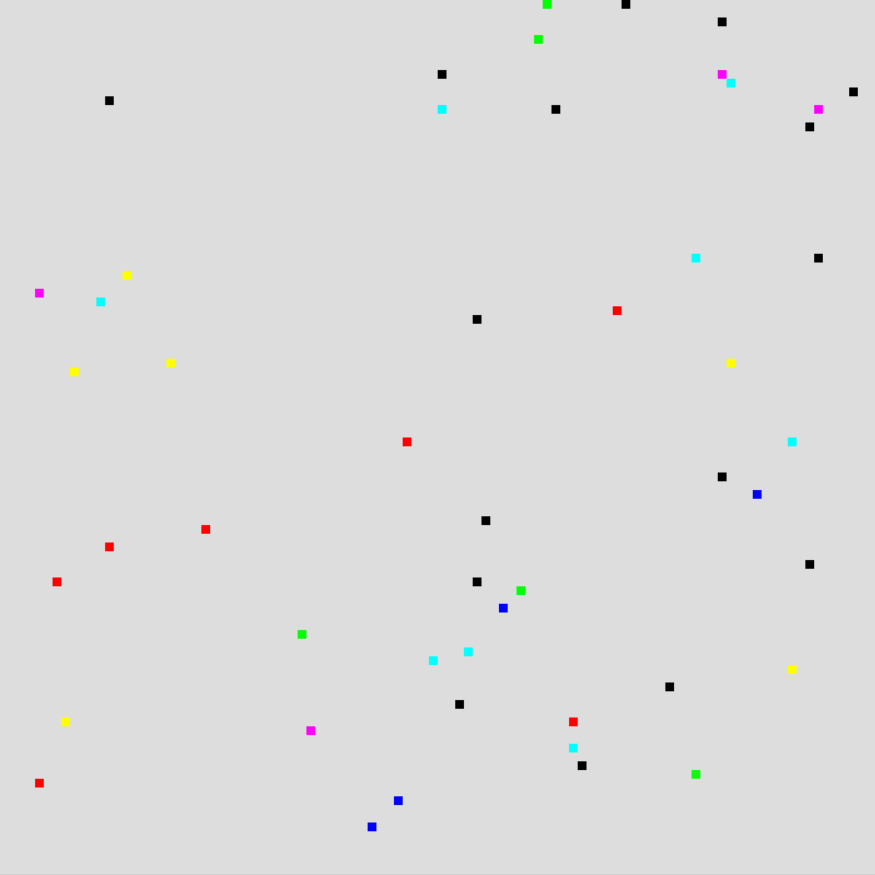
\includegraphics[width=150px]{particles}
\end{center}

\addcontentsline{toc}{subsection}{Configuration}
\subsection*{Configuration}
\begin{itemize}
\item \textbf{nbBalls}: Nombre de balles
\item \textbf{bounceBehavior}: Comportement des balles quand elles rebondissent entre-elles. SWAP; REVERSE; WAIT
\item \textbf{colors.balls}: Couleurs aléatoire des balles au départ.
\item \textbf{colors.hit}: Couleur des balles ayant eu une collision avec une autre.
\end{itemize}

\addcontentsline{toc}{subsection}{Questions}
\subsection*{Questions}
\subsubsection*{Question 1}
La simulation tourne à 1 fps avec environ 500 000 agents et l'affichage activé sans grille sur mon ordinateur. La performance va dépendre beaucoup de la machine sur laquelle le programme tourne.
\subsubsection*{Question 2}
\begin{center}
Environnements non-toriques, de tailles 10x10, 100x100 et 1000x1000 avec 50 balles, scheduler équitable
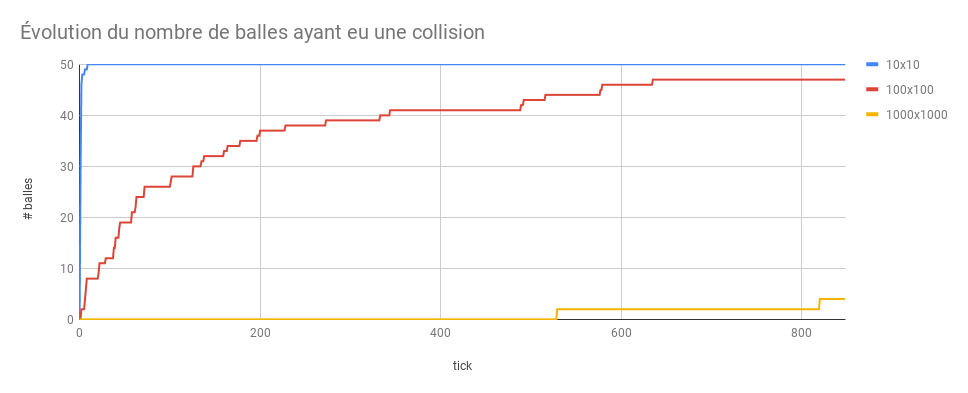
\includegraphics[width=480px]{particles_collisions}
\end{center}

\newpage

\subsubsection*{Question 3}
Avec le comportement ''Attendre si une balle me bloque'' (\textbf{bounceBehavior = WAIT}), les balles se déplacent plus lentement et si deux balles avec des directions opposées se rentre dedans elles restent bloquées en attendant l'une l'autre que l'autre bouge.\\
Avec le comportement ''Rebondir en inversant ma direction'' (\textbf{bounceBehavior = REVERSE}), si une balle va dans la même direction qu'une autre balle qui est dans la case devant elle, elle rebondira si son tour arrive avant celle de devant, mais elle ne rebondira pas sinon, car la balle se sera déplacée d'une case de plus entre temps.\\
Avec le comportement ''Rebondir en inversant ma direction avec l'autre balle'' (\textbf{bounceBehavior = SWAP}), on obtient une vrai impression de rebond.

\addcontentsline{toc}{subsection}{Difficultés techniques \& limites}
\subsection*{Difficultés techniques \& limites}
Dans la première version du TP1 il n'y avait presque pas d'architecture, et j'ai eu plein de problèmes de comportements étranges dûs à un code mal organisé. Lorsque j'ai réimplémenté le TP1 avec l'architecture complète cela m'a pris 15 minutes.

\addcontentsline{toc}{subsection}{Améliorations possibles}
\subsection*{Améliorations possibles}
Ajout d'un comportement de rebond où chaque balle calcule le vecteur milieu des deux directions comme leur nouvelle direction.\\
Dans la première version j'avais ajouté un tracé de déplacement derrière les balles, ça devrait être facile à réimplémenter avec les \textbf{Layer}.


\newpage

\addcontentsline{toc}{section}{Implémentation 2 : Wator}
\section*{Implémentation 2 : Wator}

\begin{center}
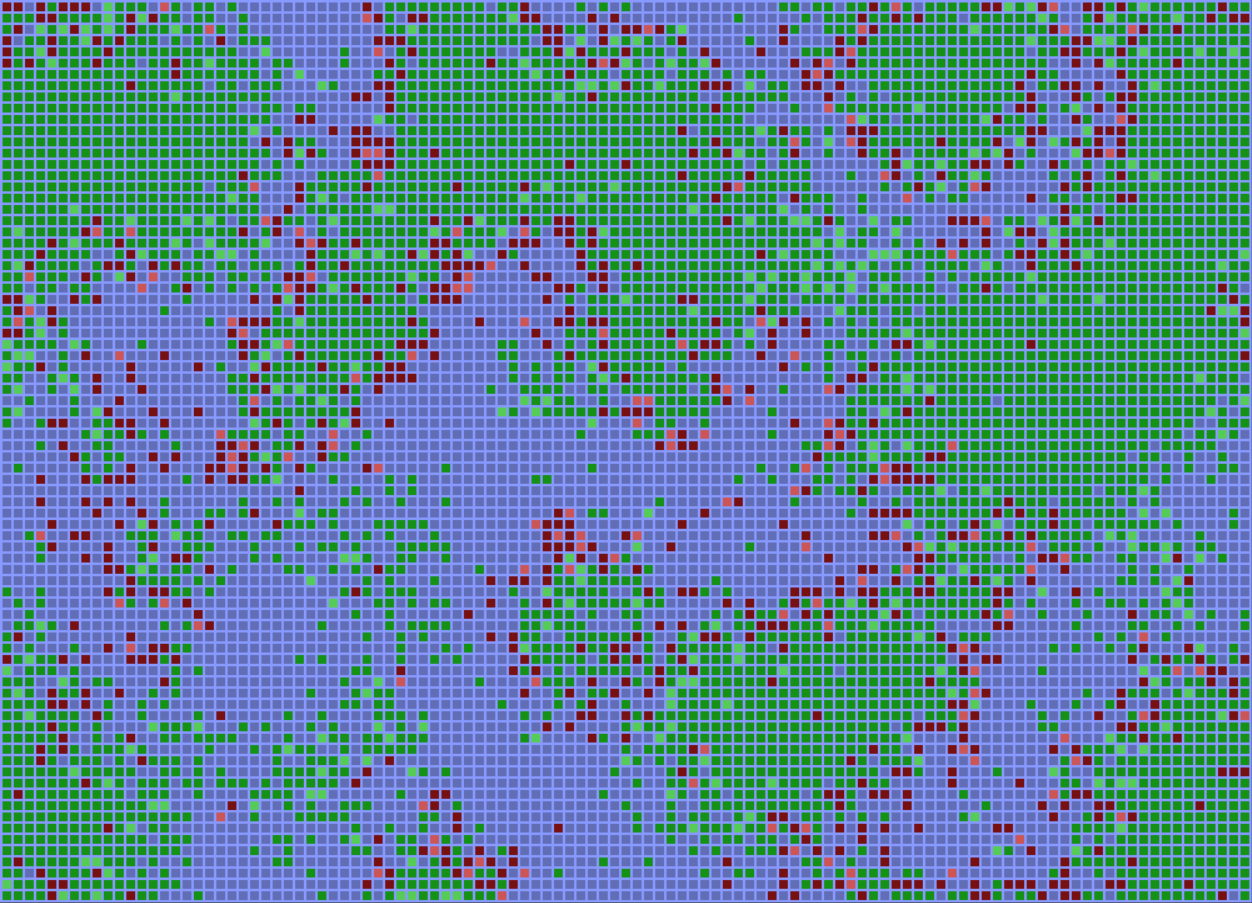
\includegraphics[width=272px]{wator}
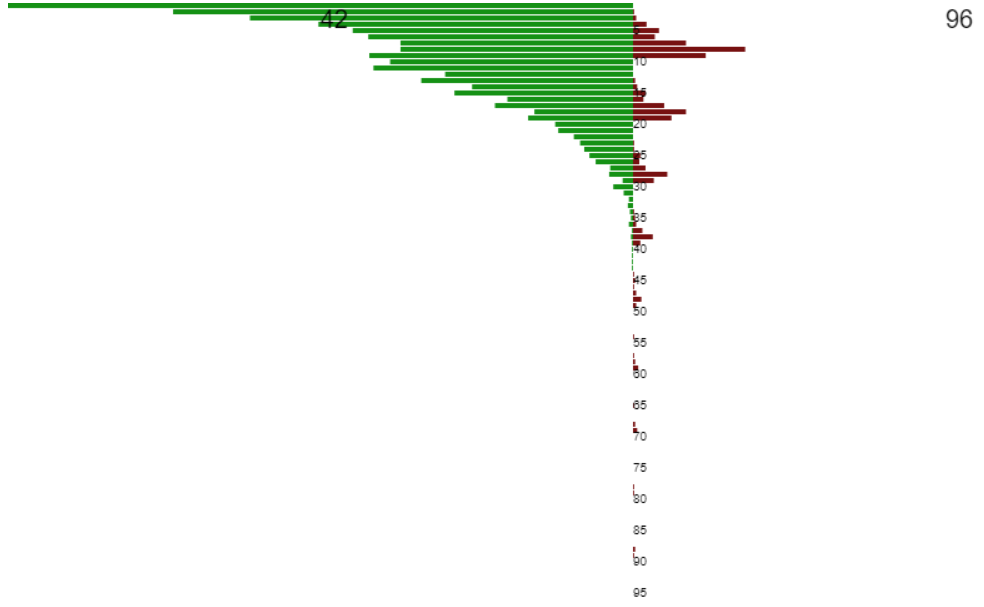
\includegraphics[width=200px, height=195px]{watorpyramid}
\end{center}

\addcontentsline{toc}{subsection}{Configuration}
\subsection*{Configuration}
\begin{itemize}
\item \textbf{nbFish}: Nombre de poissons
\item \textbf{nbSharks}: Nombre de requins
\item \textbf{fishGestation}: Temps (minimum si \textbf{randomGestation}) nécessaire pour faire naître un poisson
\item \textbf{sharkGestation}: Temps (minimum si \textbf{randomGestation}) nécessaire pour faire naître un requin
\item \textbf{sharkStarvation}: Temps (minimum si \textbf{randomStarvation}) nécessaire pour qu'un requin meure de faim
\item \textbf{babySharkFood}: Temps (minimum si \textbf{randomStarvation}) nécessaire pour qu'un requin qui n'a encore jamais mangé meure
\item \textbf{randomGestation}: Si vrai, le temps de gestation est aléatoire
\item \textbf{fishGestationRange}: Variabilité du temps nécessaire pour faire naître un poisson
\item \textbf{sharkGestationRange}: Variabilité du temps nécessaire pour faire naître un requin
\item \textbf{randomStarvation}: Si vrai, le temps pour mourir de faim est aléatoire
\item \textbf{sharkStarvationRange}: Variabilité du temps nécessaire pour qu'un requin meure de faim
\item \textbf{babySharkFoodRange}: Variabilité du temps nécessaire pour qu'un requin qui n'a encore jamais mangé meure
\item \textbf{oneActionPerTurn}: Si vrai, les agents ne peuvent faire d'une action par tour parmis bouger, manger (et bouger si \textbf{moveWhenEating}) et se reproduire.
\item \textbf{sharkReproduceWhenEating}: Si vrai, les requins peuvent se reproduire quand ils mangent
\item \textbf{sharkReproduceWhenMoving}: Si vrai, les requins peuvent se reproduire quand ils se déplacent sans manger
\item \textbf{moveWhenEating}: Si vrai, les agents se déplacent sur leur proie quand ils mangent
\item \textbf{fishSuffocate}: Si vrai, les poissons peuvent mourir par asphyxie
\item \textbf{fishBreath}: Le nombre de cases voisines libres nécessaires pour qu'un poisson respire
\item \textbf{explosivePregnancy}: Si vrai, quand un agent fini sa gestation mais n'est pas capable de créer un bébé, il meure et ne laisse pas d'enfant
\item \textbf{sharkGestateOnlyWhenEating}: Si vrai, les requins ne comptent comme de la gestation que les tours où ils mangent
\end{itemize}

\addcontentsline{toc}{subsection}{Questions}
\subsection*{Questions}
\subsubsection*{Question 1}
Plus l'aléatoire joue un rôle important, plus le risque qu'une simulation finisse en extermination est grand. Il faut également faire attention à ce que les requins ne naissent pas plus vite qu'ils meurent de faim sinon ils survivront même sans poissons. Pour palier à cela j'ai ajouté le paramètre \textbf{sharkGestateOnlyWhenEating} qui transforme le temps de gestation en un nombre de poissons à consommer pour accoucher.
\subsubsection*{Question 2}
Je vais comparer les comportements avec les mêmes paramètres simples. Environnement 100x100 torique, pas d'aléatoire, \textbf{fishSuffocate}, \textbf{explosivePregnancy}, \textbf{sharkGestateOnlyWhenEating} à faux et \textbf{moveWhenEating} à vrai.\\
\textbf{nbFish} = 2000, \textbf{nbSharks} = 50, \textbf{fishGestation} = 2, \textbf{sharkGestation} = 10, \textbf{sharkStarvation} = 3, \textbf{babySharkFood} = 3

\begin{center}
Situation initiale : \textbf{oneActionPerTurn} = false, \textbf{sharkReproduceWhenEating} = true, \textbf{sharkReproduceWhenMoving} = true
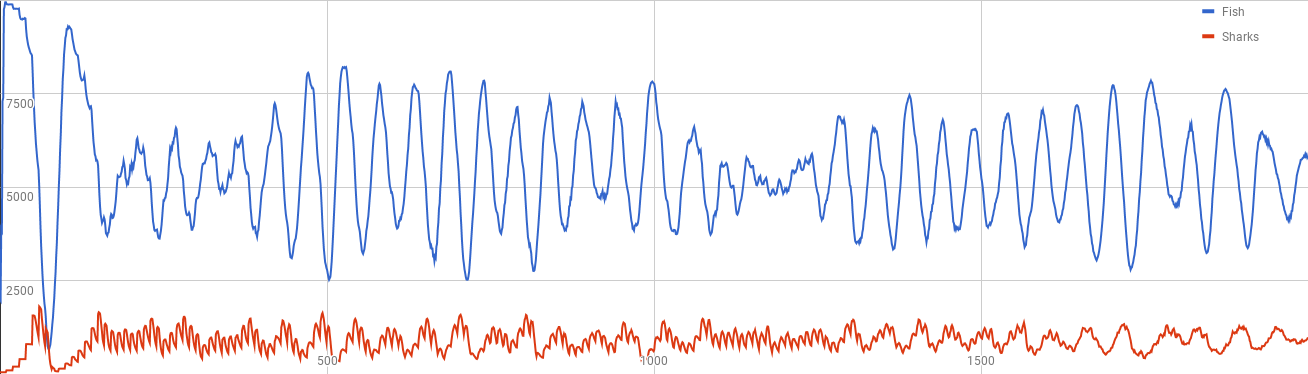
\includegraphics[width=500px]{wator_0}\\
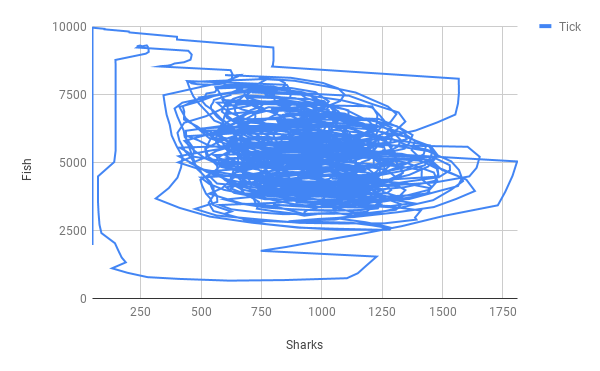
\includegraphics[width=250px]{wator_0b}
\end{center}

En observant la courbe on remarque qu'il y a une période de stabilisation au début de la simulation dû à une oscillation d'un trop grand nombre de poissons qui nourissent un trop grand nombre de requins qui mangent un trop grand nombre de poissons ce qui affame les requins, etc... Jusqu'à avoir une oscillation stable.
En observant la simulation on remarque que les bancs de poissons sont définis par les requins qui les encerclent. Ces bancs rétrécissent au fur et à mesure que les requins les mangent mais les poissons se reproduisent plus vite et un autre banc se créé avant que le premier ne disparaisse.

Dans la situation 1, dû au fait que les poissons n'ont que 2 actions et les requins 3, les poissons prennent rapidement tout l'espace disponible, et une fois cela fait, un requin n'a pas l'occasion d'accoucher car il n'y a jamais de place puisque la case qu'il a mangé est déjà remplie.\\
Les requins ne meurent donc jamais mais ne font aucun enfant.

\newpage

\begin{center}
Situation 1 : \textbf{oneActionPerTurn} = true
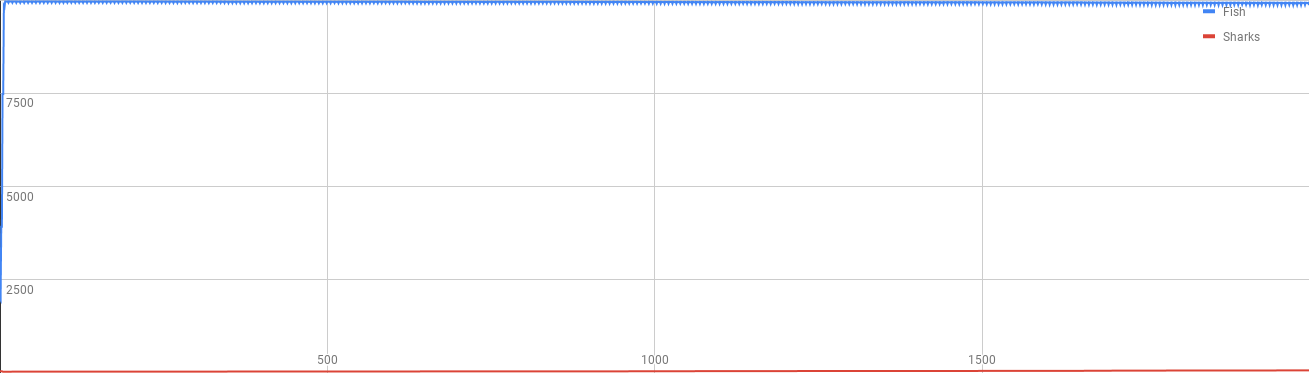
\includegraphics[width=450px]{wator_1}\\
\end{center}

Si on compense cela en augmentant le temps de gestation des poissons, on arrive à une situation où éventuellement il y a suffisemment de requins les uns à coté des autres pour que certains mangent un poisson et d'autres accouchent, et à un moment donné des bancs de poissons commencent à apparaître. Cependant il faut un certain temps pour arriver à cet état car il faut que les requins soient bien synchronisés.
\begin{center}
Situation 1 bis : \textbf{oneActionPerTurn} = true, \textbf{fishGestation} = 8
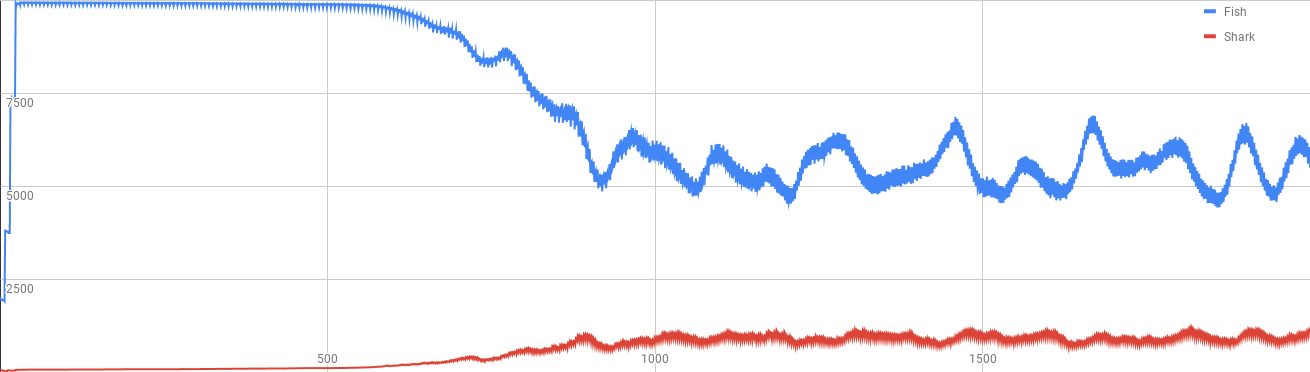
\includegraphics[width=450px]{wator_1bis}\\
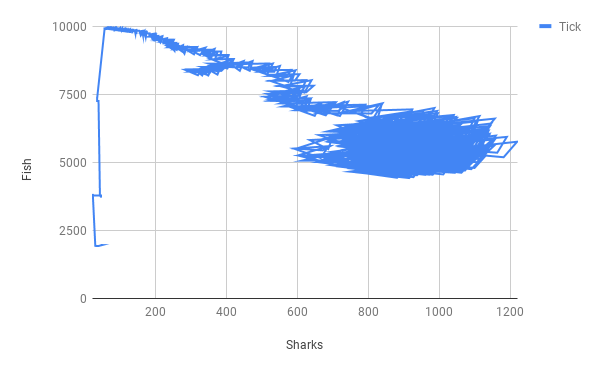
\includegraphics[width=250px]{wator_1bisb}
\end{center}
Dans cet état, on remarque une différence notable, les bancs de poissons se déplacent pendant une longue période sans requins autour, car ceux-ci n'ont pas encore eu le temps de les rattrapper, ce qui donne un côté plus naturel à la simulation par rapport à la situation initiale.\\

Un effet similaire se produit dans la situation 2, à la différence près que même en augmentant le temps de gestation des poissons, les requins n'arrivent jamais à se reproduire car ils mangent tout le temps et donc ne bougent jamais sans manger.
\begin{center}
Situation 2 : \textbf{oneActionPerTurn} = false, \textbf{sharkReproduceWhenEating} = false, \textbf{sharkReproduceWhenMoving} = true
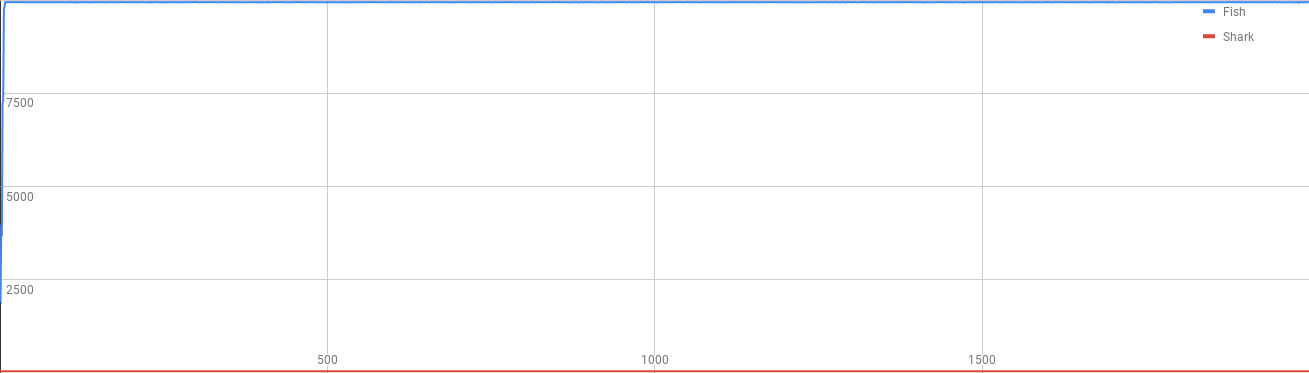
\includegraphics[width=450px]{wator_2}
\end{center}

\newpage

Dans la situation 3, les bébés requins naissent uniquement aux abords des bancs de poissons, mais à part cela il n'y a pas de différence notable avec la situation initiale sauf peut-être des variations légèrement plus douces comme le montre l'apparence plus arrondie de la courbe des poissons sur les requins.
\begin{center}
Situation 3 : \textbf{oneActionPerTurn} = false, \textbf{sharkReproduceWhenEating} = true, \textbf{sharkReproduceWhenMoving} = false
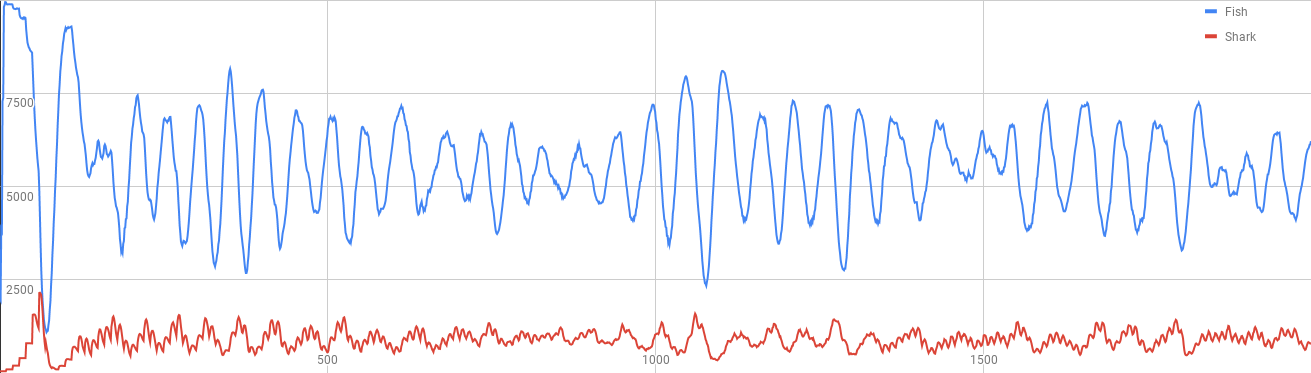
\includegraphics[width=500px]{wator_3}\\
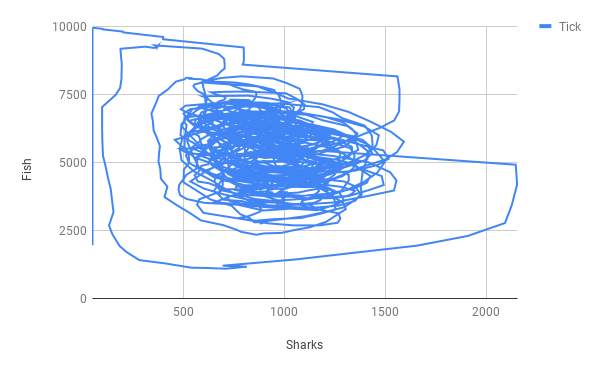
\includegraphics[width=300px]{wator_3b}
\end{center}

\addcontentsline{toc}{subsection}{Difficultés techniques \& limites}
\subsection*{Difficultés techniques \& limites}
La possibilité de supprimer et d'ajouter des agents est passée par plusieurs itérations. D'abord avec des listes d'agents séparés, mais les agents devaient à la fois immédiatement disparaître et apparaître dans l'environnement mais également ne pas jouer leur tour si ils sont morts ou nouveaux-nés. J'ai donc mis en place le système actuel où les agents sont marqués à leur mort et leur naissance, et répondent donc false à l'appel de \textbf{isActive()}.

\addcontentsline{toc}{subsection}{Améliorations possibles}
\subsection*{Améliorations possibles}
Comme il ya beaucoup de paramètres modifiables, les nombre de combinaisons de situations est gigantesque, et il est difficile de les comparer car il faut à chaque fois faire des petites modifications et redémarer la simulation pour voir ce que ça change.\\
Il faudrait donc pouvoir modifier certains paramètres pendant l'éxécution pour pouvoir plus facilement expérimenter.

\newpage

\addcontentsline{toc}{section}{Implémentation 3 : Pacman}
\section*{Implémentation 3 : Pacman}

\begin{center}
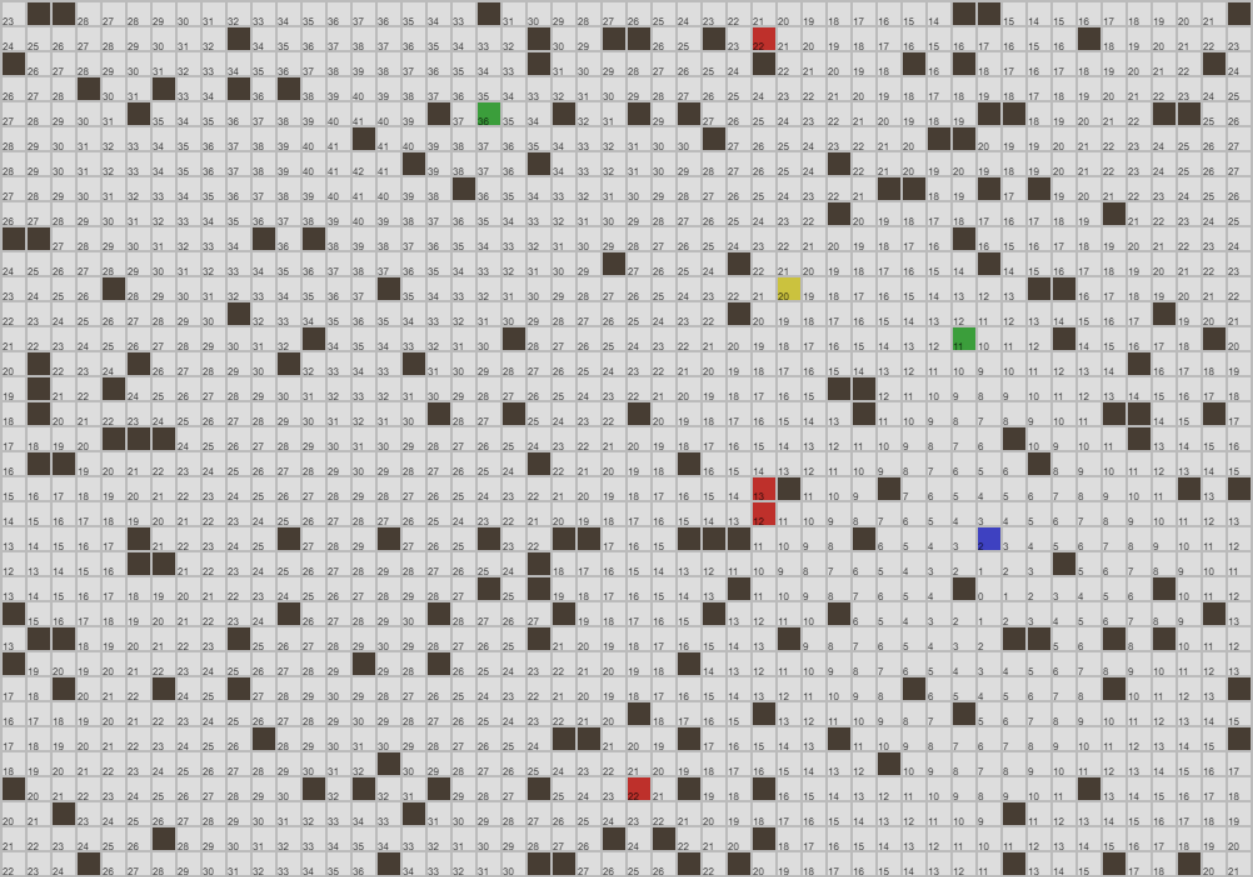
\includegraphics[width=350px]{pacman}
\end{center}

\addcontentsline{toc}{subsection}{Configuration}
\subsection*{Configuration}
\begin{itemize}
\item \textbf{wallProbability}: Probabilité de placer un mur sur une case
\item \textbf{nbGhosts}: Nombre de fantômes
\item \textbf{nbPowerpellets}: Nombre de pastilles
\item \textbf{playerSpeed}: Vitesse du joueur (1 - 100)
\item \textbf{ghostSpeed}: Vitesse des fantômes (1 - 100)
\item \textbf{powerpelletDurationFactor}: Facteur qui, multiplié par le nombre de cases de l'environnement, donne la durée de vie d'une pastille
\item \textbf{powerpelletStrength}: Durée d'invincibilité donné par une pastille
\item \textbf{overload}: Nombre de pastilles à avaler pour ouvrir une sortie
\end{itemize}

\addcontentsline{toc}{subsection}{Comportements}
\subsection*{Comportements}
J'ai remarqué que lorsque le joueur se déplace trop vite, on est beaucoup moins précis dans nos déplacement et cela rend le jeu beaucoup plus difficile même si les fantômes sont lents. Plus l'espace de jeu est grand, plus c'est facile d'échapper aux fantômes. Un jeu dans un environnement non-torique est presque impossible à gagner.\\

\addcontentsline{toc}{subsection}{Difficultés techniques \& limites}
\subsection*{Difficultés techniques \& limites}
Lorsqu'il a fallut introduire la notion d'input, j'ai dû complètement repenser l'architecture pour en faire ce qu'elle est aujourd'hui. En JS il n'y a pas de compilation, donc c'est facile d'oublier quelque chose en réfactorant sur une grosse architecture comme celle-ci. Et lorsqu'il y a une erreur, elle n'est pas indiquée, il faut beaucoup creuser pour comprendre pourquoi une variable se retrouve avec la valeur undefined.\\
J'ai aussi passé beaucoup de temps à trouver une architecture convenable pour gérer les inputs, en effet, en JS on dépend du contexte de la page web pour récupérer les inputs. Or je voulais que le contexte web reste séparé de l'architecture tout en communiquant les events aux agents.\\
Au final la solution fut de créer la classe \textbf{EventQueue} qui est remplie d'event par des listeners placés sur le DOM par \textbf{MultiAgentSystem} et dont on passe une référence à l'agent pour qu'il puisse lire les events sur la pile.\\

\addcontentsline{toc}{subsection}{Améliorations possibles}
\subsection*{Améliorations possibles}
J'aurais bien voulu essayer de générer un labyrinthe aléatoire, voire même d'avoir une phase où des \textbf{WallAgent} se déplacent en suivant leur logique propre et créent un labyrinthe par émergence à la manière des tas des termites.\\
Il serait aussi intéressant d'avoir plusieurs niveau d'IA des fantômes. En cours de développement j'ai amélioré l'IA, mais je n'ai pas laissé l'option de jouer avec la version simple.\\
La version simple fait qu'un fantôme qui cherche la prochaine case parcourera les cases de son environnement toujours dans le même ordre, ce qui fait que si il y a 2 cases avec la même valeur (ce qui est souvent le cas), il prendra toujours la même (par exemple celle avec les x y les plus petits). Dans la version améliorée je mélange l'ordre de parcours des cases voisines, et le résultat est incroyablement imprévisible et cela rend très difficile l'attaque de fantôme en mode invincible.

\end{document}